%-----------------------------------------------------------------------------%
\chapter{\topikSatu}
%-----------------------------------------------------------------------------%

%-----------------------------------------------------------------------------%
\section{Pendahuluan}
%-----------------------------------------------------------------------------%
Topik eksperimen pertama adalah perkalian matriks-vektor dan perkalian matriks bujur sangkar dengan beberbagai algoritma paralel. 

\subsection{Perkalian Matriks-Vektor} 

\subsubsection{Row-Wise Decomposition}

Algoritma paralel perkalian matriks-vektor yang paling sederhana, yaitu memecah proses perkalian berdasarkan baris matriks (\f{row-wise}). Setiap prosesor akan bertanggung jawab untuk mengalikan sebuah baris matriks dan vektor pada satu waktu. Jika jumlah prosesor ($np$) lebih sedikit dari jumlah baris matriks ($r$) maka setiap prosesor bertugas mengalikan $n = \frac{r}{np}$ secara sekuensial.

\begin{figure}
	\centering
	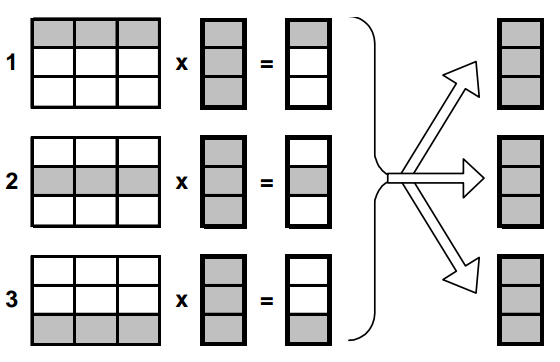
\includegraphics[width=0.75\textwidth]
	{pics/mv_rowwise}
	\caption{Perkalian matriks-vektor Row-Wise Decomposition}
	\label{fig:mv_rowwise}
\end{figure}  

\subsubsection{Column-wise Decomposition}

Algoritma perkalian matriks-vektor ini merupakan alternatif dari \f{row-wise decomposition} di mana pemecahan proses perkalian dilakukan berdasarkan kolom matriks. Setiap proses akan mengalikan sebuah kolom matriks dan sebuah elemen vektor pada satu waktu. Mirip dengan algoritma \f{row-wise decomposition}, jika jumlah prosesor ($np$) lebih sedikit dari jumlah kolom matriks ($c$) maka setiap prosesor bertugas mengalikan $n = \frac{c}{np}$ secara sekuensial.

\begin{figure}
	\centering
	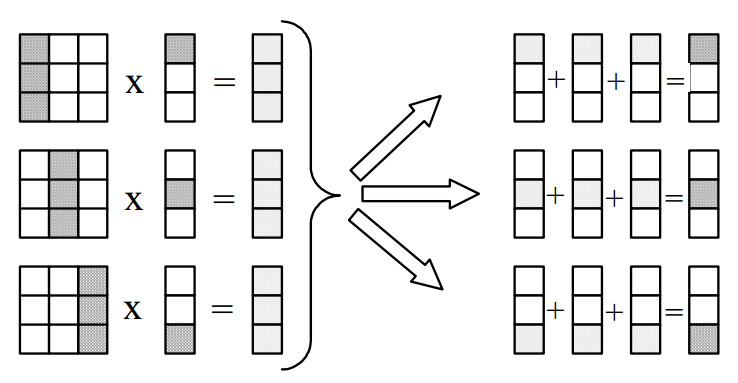
\includegraphics[width=0.9\textwidth]
	{pics/mv_colwise}
	\caption{Perkalian matriks-vektor Column-Wise Decomposition}
	\label{fig:mv_colwise}
\end{figure}  

\subsubsection{Checkerboard Decomposition}

Algoritma perkalian matriks-vektor \f{checkerboard decomposition} ini membagi matriks menjadi submatriks dengan ukuran yang sama dan mengalikannya dengan subvektor yang sesuai. Hasil perkalian tersebut kemudian akan dijumlahkan dan dipetakan ke vektor hasil.

Prekondisi dari algoritma ini adalah jumlah elemen matriks ($n$) harus bisa dibagi rata ke sejumlah prosesor ($np$) atau dengan kata lain memenuhi persamaan \ref{eq:mv_checkerboard}. Hasil pembagian ini ($x$) akan menjadi ukuran submatriks (dan subvektor) yang dikerjakan di tiap proses secara paralel.

\begin{equation}
	x = \sqrt{\frac{n}{np}},\text{ where } x \in \mathbb{Z}
	\label{eq:mv_checkerboard}
\end{equation}


\begin{figure}
	\centering
	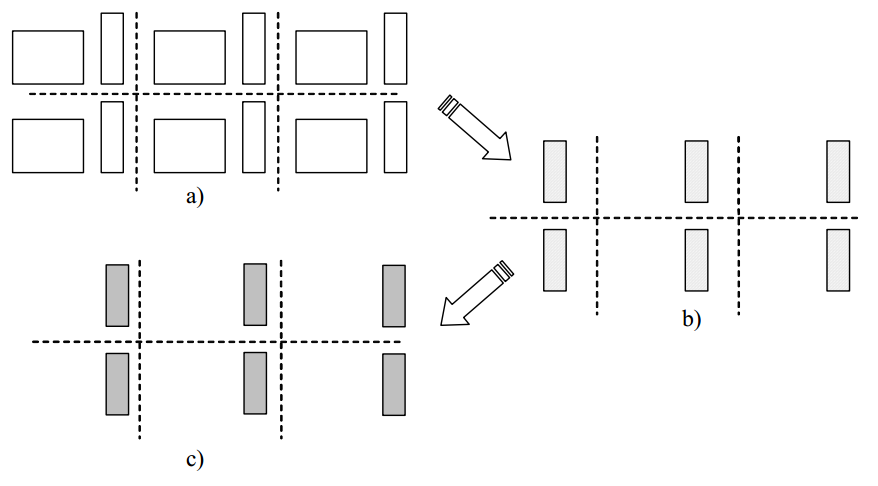
\includegraphics[width=0.75\textwidth]
	{pics/mv_checkerboard}
	\caption{Perkalian matriks-vektor Checkerboard Decomposition}
	\label{fig:mv_checkerboard}
\end{figure}  

\subsection{Perkalian Matriks Bujursangkar} 

\subsubsection{Row-Wise Decomposition}

Mirip dengan algoritma perkalian matriks-vektor \f{row-wise decomposition}, algortima ini juga membagi pekerjaan berdasarkan baris dari matriks pertama seperti yang diilustrasikan pada gambar \ref{fig:mm_rowwise}. Setiap prosesor akan mengalikan sebuah baris dari matriks pertama $A$ dengan seluruh kolom dari matriks kedua $B$. Hasil dari seluruh prosesor kemudian dikonkatenasi menjadi matriks baru $C$.

\begin{figure}
	\centering
	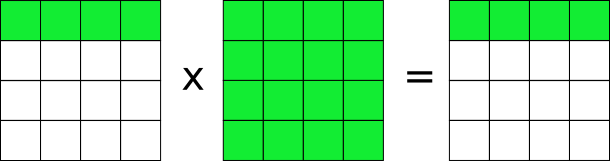
\includegraphics[width=1\textwidth]
	{pics/mm_rowwise}
	\caption{Perkalian matriks bujursangkar Row-Wise Decomposition}
	\label{fig:mm_rowwise}
\end{figure}

\subsubsection{Cannon}

Algoritma Cannon menggunakan dekomposisi seperti algortima matriks-vektor \f{checkerboard decomposition} di mana matriks $A$ dan $B$ dibagi menjadi menjadi submatriks bujursangkar. Perbedaan pada algoritma Cannon adalah prekondisi di mana jumlah proses ($np$) harus merupakan bujursangkar sempurna (\f{perfect square}). Tujuan utama dari algoritma ini adalah untuk meningkatkan efisiensi penggunaan memori pada proses paralel.

\begin{figure}
	\centering
	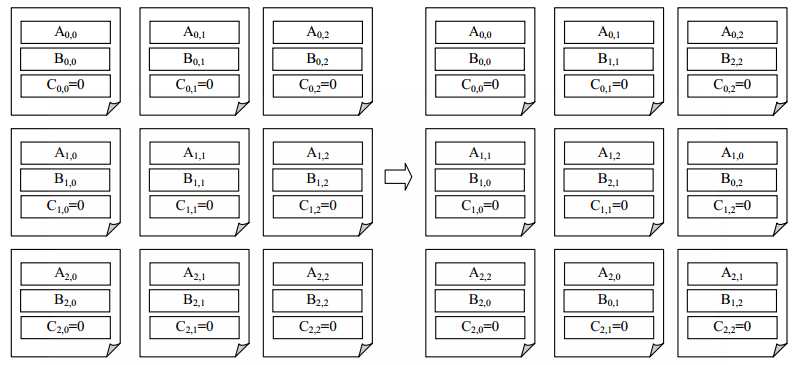
\includegraphics[width=1\textwidth]
	{pics/mm_cannon}
	\caption{Perkalian matriks bujursangkar Cannon}
	\label{fig:mm_cannon}
\end{figure}

\subsubsection{Fox}

Algoritma Fox memiliki kemiripan dengan algoritma Cannon dalam hal dekomposisi matriks menjadi submatriks bujursangkar dan pemetaan prosesor yang harus dapat membentuk bujursangkar sempurna (\f{perfect square}). Yang membedakan algoritma Fox dan Cannon adalah skema distribusi awal submatriks ke prosesor

\begin{figure}
	\centering
	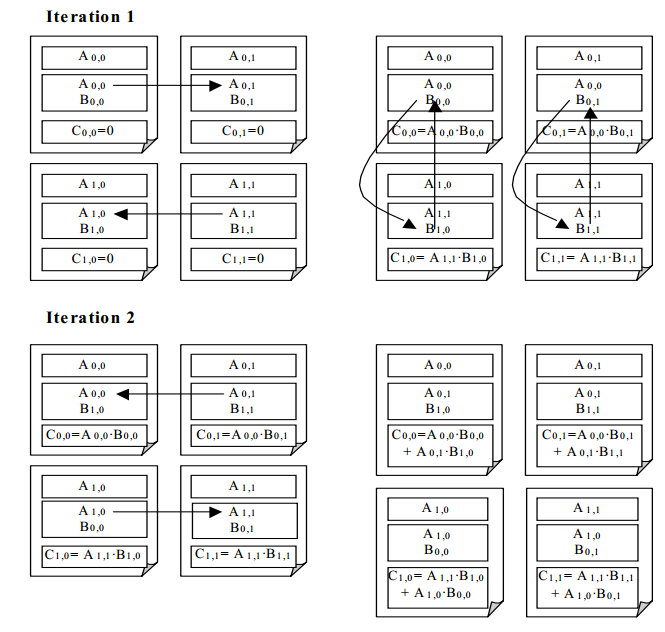
\includegraphics[width=0.75\textwidth]
	{pics/mm_fox}
	\caption{Perkalian matriks bujursangkar Fox}
	\label{fig:mm_fox}
\end{figure}

\subsubsection{DNS}

Algoritma yang diberi nama berdasarkan nama pembuatnya (Dekel, Nassimi and Aahni) ini, diajukan dalam rangka meningkatkan lagi efisiensi penggunaan memori pada perkalian matriks bujursangkar secara paralel. Karakteristik algoritma ini adalah:
\begin{itemize}
	\item Berdasarkan partisi \f{intermediate data}
	\item Melakukan perkalian skalar $n^3$ sehingga membutuhkan proses sebanyak $n \times n \times n$
	\item Membutuhkan waktu komputasi $O(\log n)$ dengan menggunakan $O(\frac{n^3}{\log n})$
\end{itemize}

\begin{figure}
	\centering
	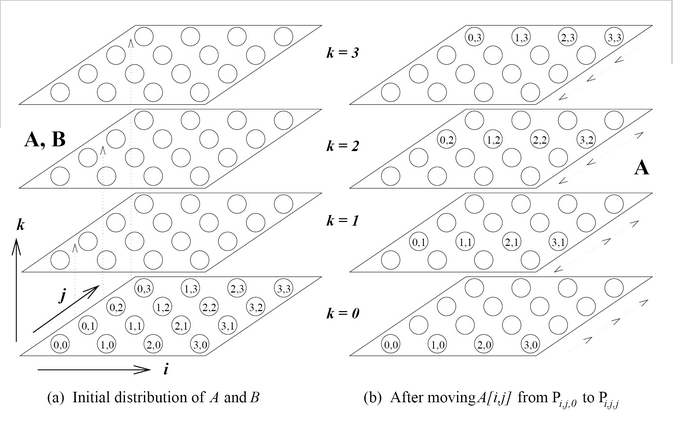
\includegraphics[width=1\textwidth]
	{pics/mm_dns1}
	\caption{Perkalian matriks bujursangkar DNS iterasi 1}
	\label{fig:mm_dns1}
\end{figure}

\begin{figure}
	\centering
	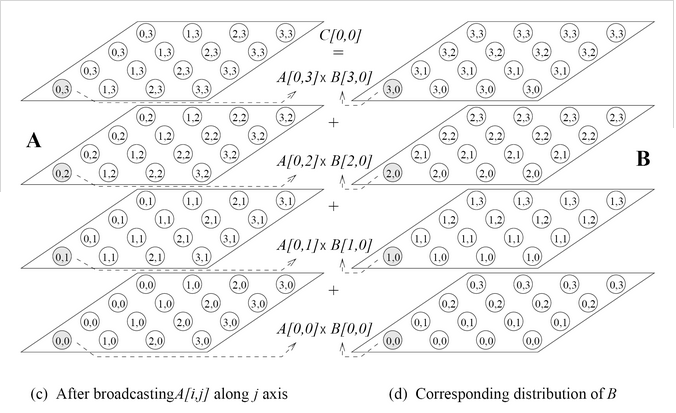
\includegraphics[width=1\textwidth]
	{pics/mm_dns2}
	\caption{Perkalian matriks bujursangkar DNS iterasi 2}
	\label{fig:mm_dns2}
\end{figure}


%-----------------------------------------------------------------------------%
\section{Eksperimen}
%-----------------------------------------------------------------------------%

\subsection{Perkalian Matriks-Vektor} 

\subsubsection{Row-Wise Decomposition}

Algoritma paralel perkalian matriks-vektor yang paling sederhana, yaitu memecah proses perkalian berdasarkan baris matriks (\f{row-wise}). Setiap prosesor akan bertanggung jawab untuk mengalikan sebuah baris matriks dan vektor pada satu waktu. Jika jumlah prosesor ($np$) lebih sedikit dari jumlah baris matriks ($r$) maka setiap prosesor bertugas mengalikan $n = \frac{r}{np}$ secara sekuensial.

\begin{figure}
	\centering
	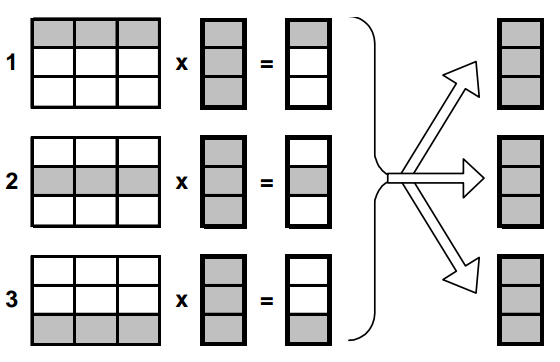
\includegraphics[width=0.75\textwidth]
	{pics/mv_rowwise}
	\caption{Perkalian matriks-vektor Row-Wise Decomposition}
	\label{fig:mv_rowwise}
\end{figure}  

\subsubsection{Column-wise Decomposition}

Algoritma perkalian matriks-vektor ini merupakan alternatif dari \f{row-wise decomposition} di mana pemecahan proses perkalian dilakukan berdasarkan kolom matriks. Setiap proses akan mengalikan sebuah kolom matriks dan sebuah elemen vektor pada satu waktu. Mirip dengan algoritma \f{row-wise decomposition}, jika jumlah prosesor ($np$) lebih sedikit dari jumlah kolom matriks ($c$) maka setiap prosesor bertugas mengalikan $n = \frac{c}{np}$ secara sekuensial.

\begin{figure}
	\centering
	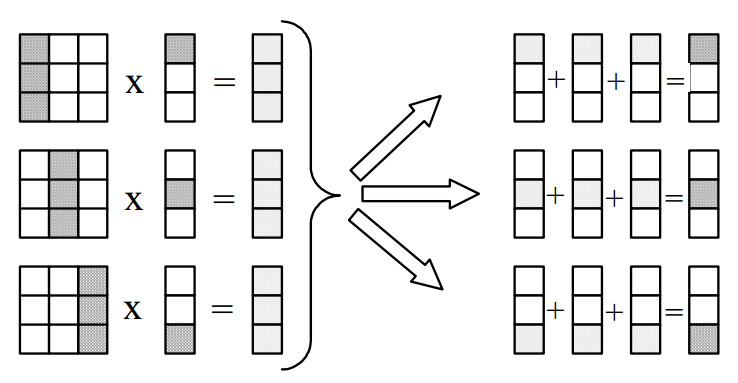
\includegraphics[width=0.9\textwidth]
	{pics/mv_colwise}
	\caption{Perkalian matriks-vektor Column-Wise Decomposition}
	\label{fig:mv_colwise}
\end{figure}  

\subsubsection{Checkerboard Decomposition}

Algoritma perkalian matriks-vektor \f{checkerboard decomposition} ini membagi matriks menjadi submatriks dengan ukuran yang sama dan mengalikannya dengan subvektor yang sesuai. Hasil perkalian tersebut kemudian akan dijumlahkan dan dipetakan ke vektor hasil.

Prekondisi dari algoritma ini adalah jumlah elemen matriks ($n$) harus bisa dibagi rata ke sejumlah prosesor ($np$) atau dengan kata lain memenuhi persamaan \ref{eq:mv_checkerboard}. Hasil pembagian ini ($x$) akan menjadi ukuran submatriks (dan subvektor) yang dikerjakan di tiap proses secara paralel.

\begin{equation}
x = \sqrt{\frac{n}{np}},\text{ where } x \in \mathbb{Z}
\label{eq:mv_checkerboard}
\end{equation}


\begin{figure}
	\centering
	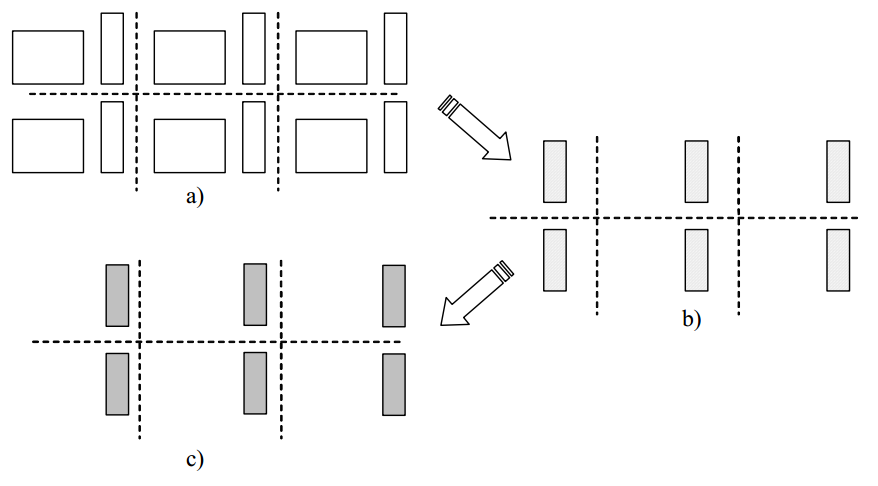
\includegraphics[width=0.75\textwidth]
	{pics/mv_checkerboard}
	\caption{Perkalian matriks-vektor Checkerboard Decomposition}
	\label{fig:mv_checkerboard}
\end{figure}  

\subsection{Perkalian Matriks Bujursangkar} 

\subsubsection{Row-Wise Decomposition}

Mirip dengan algoritma perkalian matriks-vektor \f{row-wise decomposition}, algortima ini juga membagi pekerjaan berdasarkan baris dari matriks pertama seperti yang diilustrasikan pada gambar \ref{fig:mm_rowwise}. Setiap prosesor akan mengalikan sebuah baris dari matriks pertama $A$ dengan seluruh kolom dari matriks kedua $B$. Hasil dari seluruh prosesor kemudian dikonkatenasi menjadi matriks baru $C$.

\begin{figure}
	\centering
	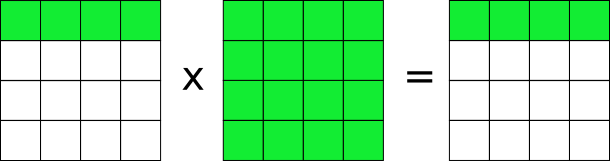
\includegraphics[width=1\textwidth]
	{pics/mm_rowwise}
	\caption{Perkalian matriks bujursangkar Row-Wise Decomposition}
	\label{fig:mm_rowwise}
\end{figure}

\subsubsection{Cannon}

Algoritma Cannon menggunakan dekomposisi seperti algortima matriks-vektor \f{checkerboard decomposition} di mana matriks $A$ dan $B$ dibagi menjadi menjadi submatriks bujursangkar. Perbedaan pada algoritma Cannon adalah prekondisi di mana jumlah proses ($np$) harus merupakan bujursangkar sempurna (\f{perfect square}). Tujuan utama dari algoritma ini adalah untuk meningkatkan efisiensi penggunaan memori pada proses paralel.

\begin{figure}
	\centering
	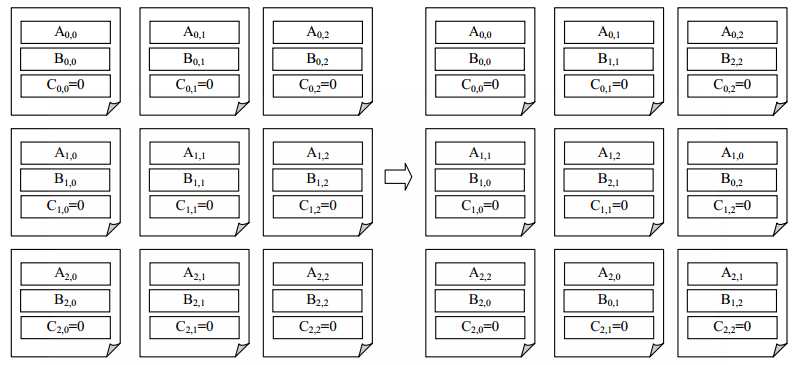
\includegraphics[width=1\textwidth]
	{pics/mm_cannon}
	\caption{Perkalian matriks bujursangkar Cannon}
	\label{fig:mm_cannon}
\end{figure}

\subsubsection{Fox}

Algoritma Fox memiliki kemiripan dengan algoritma Cannon dalam hal dekomposisi matriks menjadi submatriks bujursangkar dan pemetaan prosesor yang harus dapat membentuk bujursangkar sempurna (\f{perfect square}). Yang membedakan algoritma Fox dan Cannon adalah skema distribusi awal submatriks ke prosesor

\begin{figure}
	\centering
	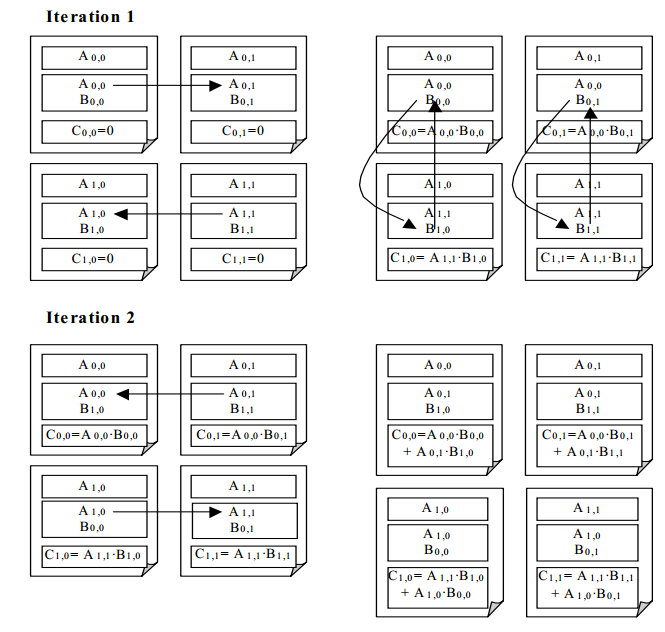
\includegraphics[width=0.75\textwidth]
	{pics/mm_fox}
	\caption{Perkalian matriks bujursangkar Fox}
	\label{fig:mm_fox}
\end{figure}

\subsubsection{DNS}

Algoritma yang diberi nama berdasarkan nama pembuatnya (Dekel, Nassimi and Aahni) ini, diajukan dalam rangka meningkatkan lagi efisiensi penggunaan memori pada perkalian matriks bujursangkar secara paralel. Karakteristik algoritma ini adalah:
\begin{itemize}
	\item Berdasarkan partisi \f{intermediate data}
	\item Melakukan perkalian skalar $n^3$ sehingga membutuhkan proses sebanyak $n \times n \times n$
	\item Membutuhkan waktu komputasi $O(\log n)$ dengan menggunakan $O(\frac{n^3}{\log n})$
\end{itemize}

\begin{figure}
	\centering
	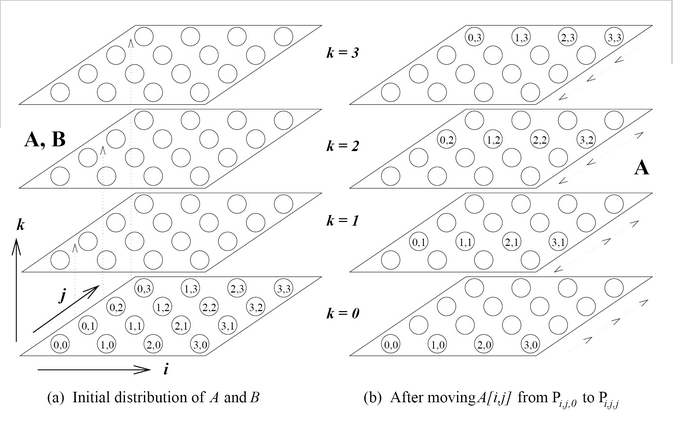
\includegraphics[width=1\textwidth]
	{pics/mm_dns1}
	\caption{Perkalian matriks bujursangkar DNS iterasi 1}
	\label{fig:mm_dns1}
\end{figure}

\begin{figure}
	\centering
	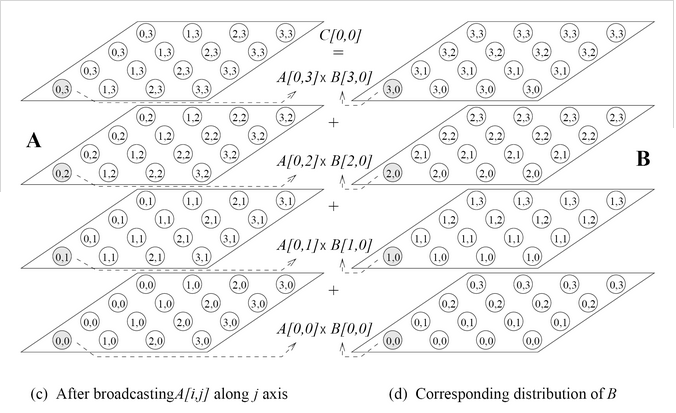
\includegraphics[width=1\textwidth]
	{pics/mm_dns2}
	\caption{Perkalian matriks bujursangkar DNS iterasi 2}
	\label{fig:mm_dns2}
\end{figure}




